\documentclass[Book Template.tex]{subfiles}
\begin{document}

    % Remove number/letter in front of Appendix
    \setcounter{secnumdepth}{-1} % levels under sublevel x are not numbered

    \chapter{Appendices}
        \label{ch: Appendices}
        \thispagestyle{noheader}

        % Cont. Remove the letter A from Table of Contents, keep the A in section numbers --------------
        \setcounter{secnumdepth}{3} % levels under sublevel x are not numbered                         |
        \setcounter{chapter}{1} % makes the module numbering start at x+1, where x is the number here  |
        % ----------------------------------------------------------------------------------------------




        
        \section{Example Figure}
            \label{app: example figure}

            \begin{figure}[!h]
                \centering
                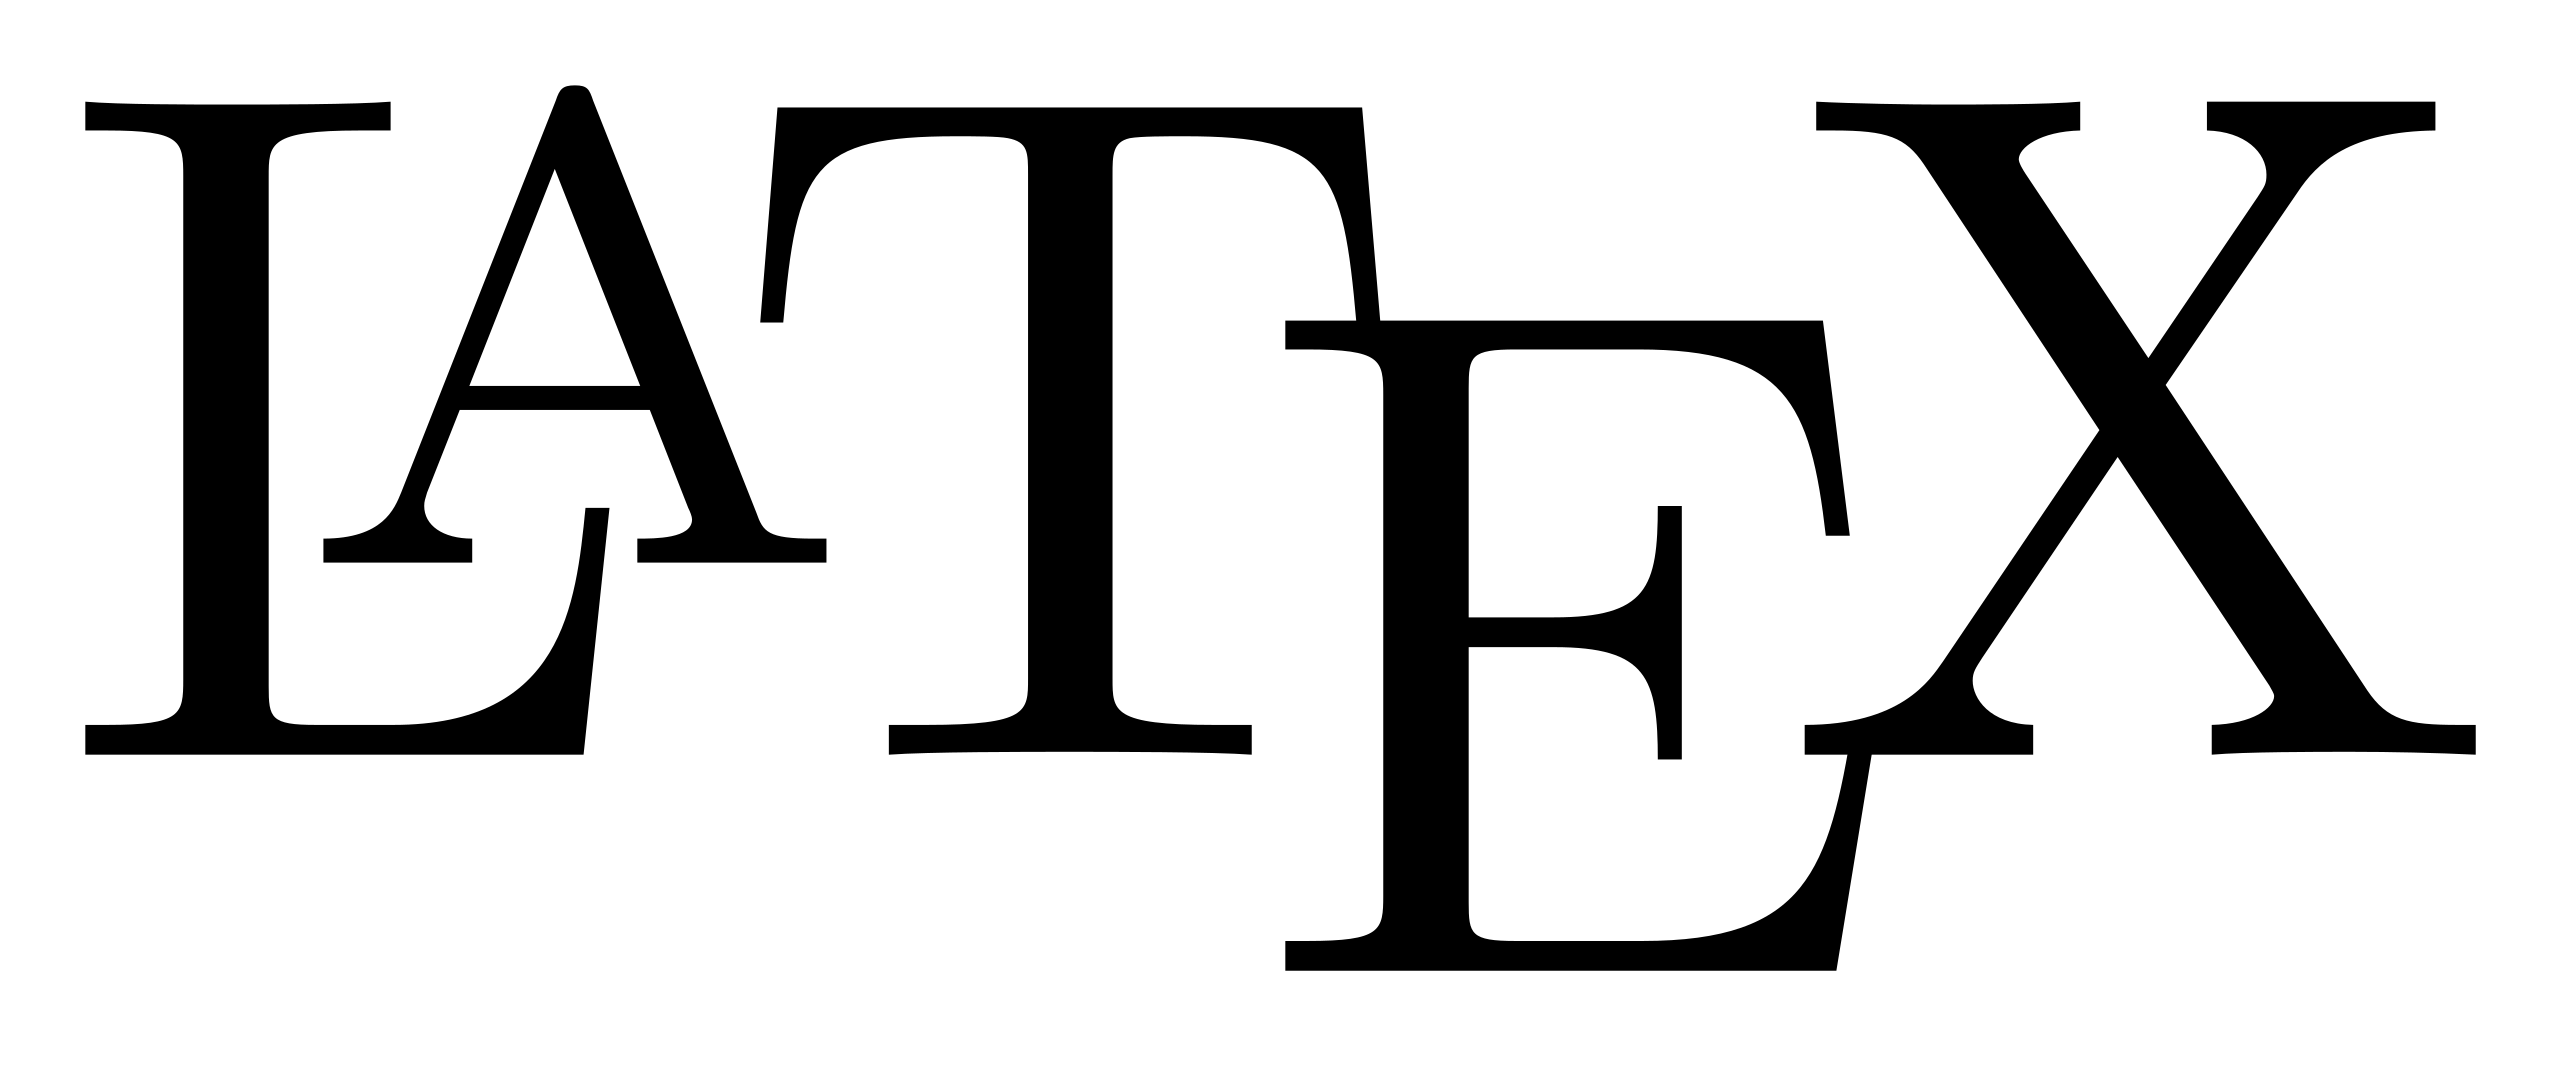
\includegraphics[width=0.5\textwidth]{LaTeX Logo.png}    

                \caption{The \LaTeX~logo. Figure captions typically go below a figure.}
                \label{fig: latex logo}
            \end{figure}

            \FloatBarrier

        \section{Example Table}
            \label{app: example table}

            \begin{table}[!h]
                \centering
                \caption{An example table. Table captions typically go above a table.}
                \label{table: example}
                \begin{tabular}{ |C{0.2\textwidth}|m{0.2\textwidth}| }
                    \hline
                    Test & text\\
                    \hline
                    \hline
                    Test & text\\
                    \hline
                    Test & text\\
                    \hline
                \end{tabular}
            \end{table}

        \section{Example Equation}
            \label{app: example equation}

            \begin{equation}
                \oiint_S \vect{E} \cdot \d\vect{A} = \frac{Q_{\text{enc}}}{\varepsilon_0}
                \label{eq: Gauss Law}
            \end{equation}
    
\end{document}

